\newpage
\section{Technosignature Searches with NenuFAR from 30-85~MHz}

This section briefly outlines ongoing efforts on carrying out the lowest frequency technosignature search to date using NenuFAR. Here a preliminary analysis is detailed which was carried out by the author and Ruaidhri Campion. It is a modified version of both the observing proposals and progress reports issued to both NenuFAR and BL teams the latter of which was led by the author. 

The technosignature observing campaign falls under the LT13 and ES13 NenuFAR programs which is led by Gregory Hellbourg at Caltech. Both programs are dedicated to high frequency resolution follow-up observations of exoplanet candidates detected with \textit{TESS}. The purpose of these observations is to search for low-frequency technosignatures from the exoplanet candidates, and to expand the multi-frequency / multi-telescope \textit{TESS} observing program led by Breakthrough Listen \citep{gsc+19}.

The nature of the program itself, aims at detect evidence of communicative extraterrestrial
civilizations, equally caters for non-exoplanet-targeted observations. As such, the team made a significant contribution into the development of a commensal acquisition pipeline allowing the collection of raw beam-formed data from any collaborating observer to be collected by the SETI back-end SETIBK. By extending observations into the 39.8–67.7 MHz frequency range, NenuFAR contributes unique low-frequency coverage that complements higher-frequency SETI surveys and broadens the search parameter space for potential technosignatures further narrowing the cosmic haystack. 

\subsection{Scientific Strategey}

The scientific strategy consists of two primary components. The first involves dedicated observations of exoplanets and \textit{TESS} targets of interest, where high-resolution beamformed data are collected and processed into Stokes-I products with fine temporal and spectral resolution to search for Doppler-drifting narrowband signals that may indicate artificial transmissions. The second component operates in a commensal mode, allowing SETI observations to be performed simultaneously with other NenuFAR scientific programs, including Exoplanets \& Stars and Cosmic Dawn, thereby maximizing telescope efficiency while significantly expanding sky coverage. In parallel, dedicated observations of the local radio frequency interference (RFI) environment are conducted to improve interference mitigation techniques essential for sensitive transient and technosignature searches.

\begin{figure}[h]
    \centering
    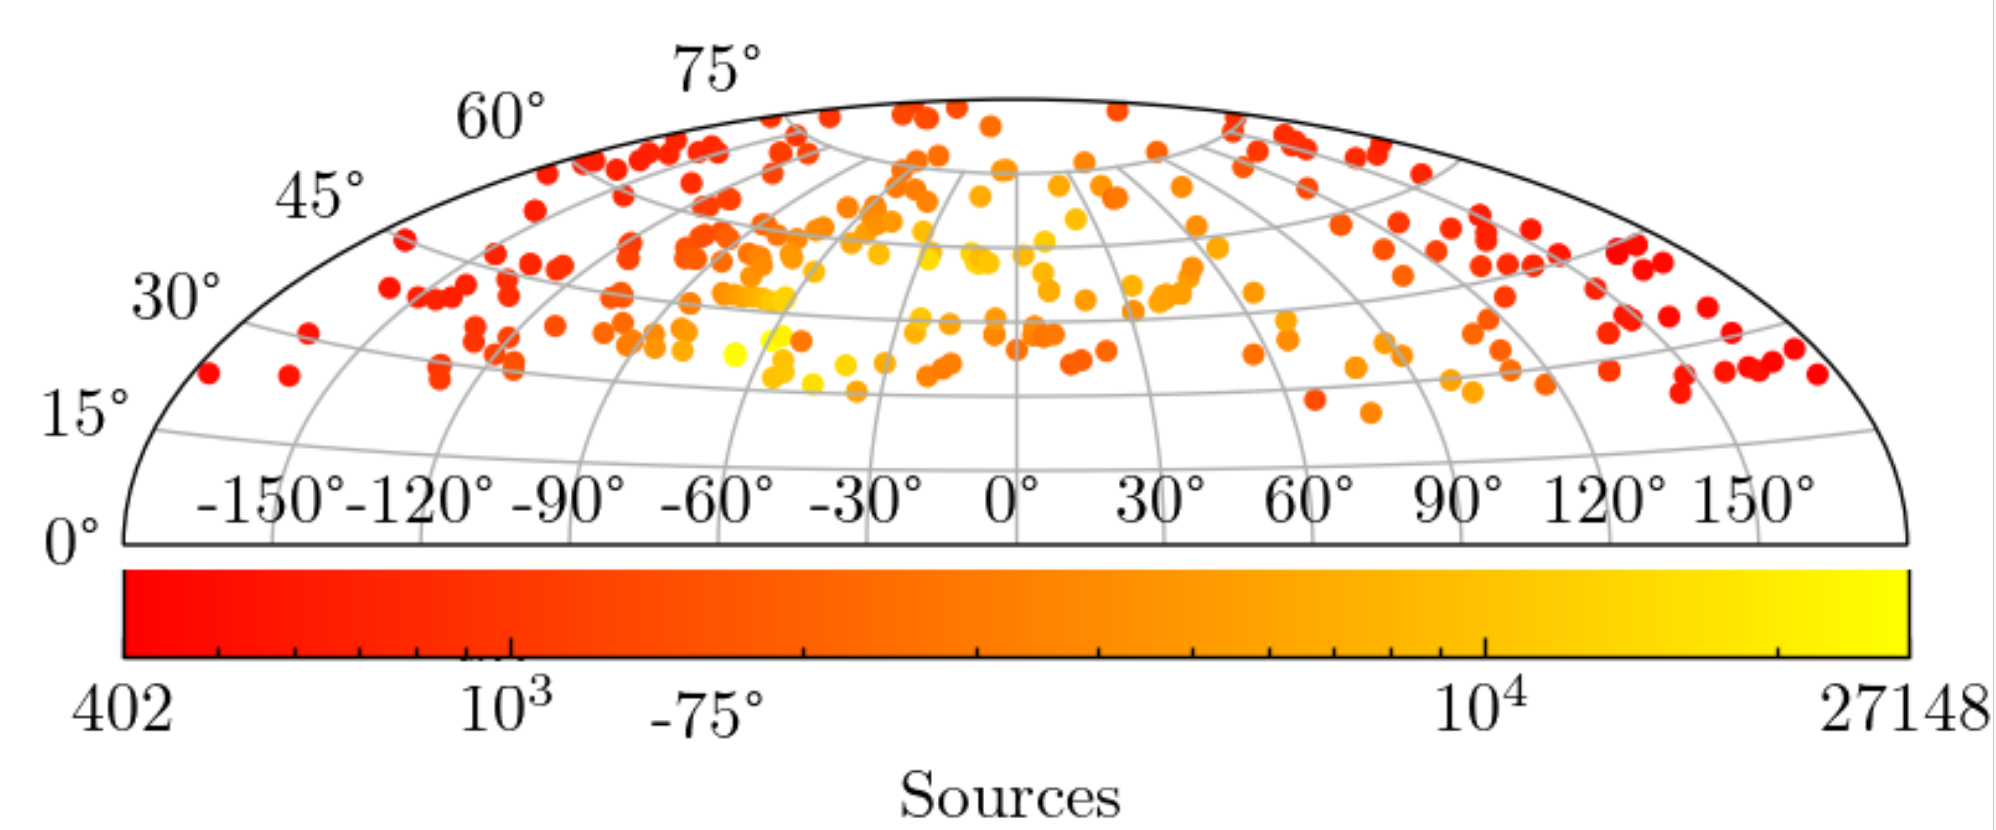
\includegraphics[width=0.6\linewidth]{chapter6/figures/NenuFAR/NenuFAR_pointings.png}
    \caption{The pointings of the NenuFAR SETI survey at the end of 2023.}
    \label{fig:NenuFAR Pointings}
\end{figure}

The observing campaign has been conducting over the last 5 years. At the end of 2023 over 297 observations of confirmed exoplanets from the NASA Exoplanet Archive (NEA) had been performed, resulting in 175 hours of raw observational data. The distribution of the points across the Northern sky is shown in \cref{fig:NenuFAR Pointings}. As with LOFTS and \cref{sec:SETIchapter} \textit{Gaia's} catalogue was searched for each of the pointings, initially identifying more than 3.5 million stellar sources before applying positional and distance uncertainty filters that reduced the effective target sample to approximately 868,665 stars.

\begin{figure}[h]
    \centering
    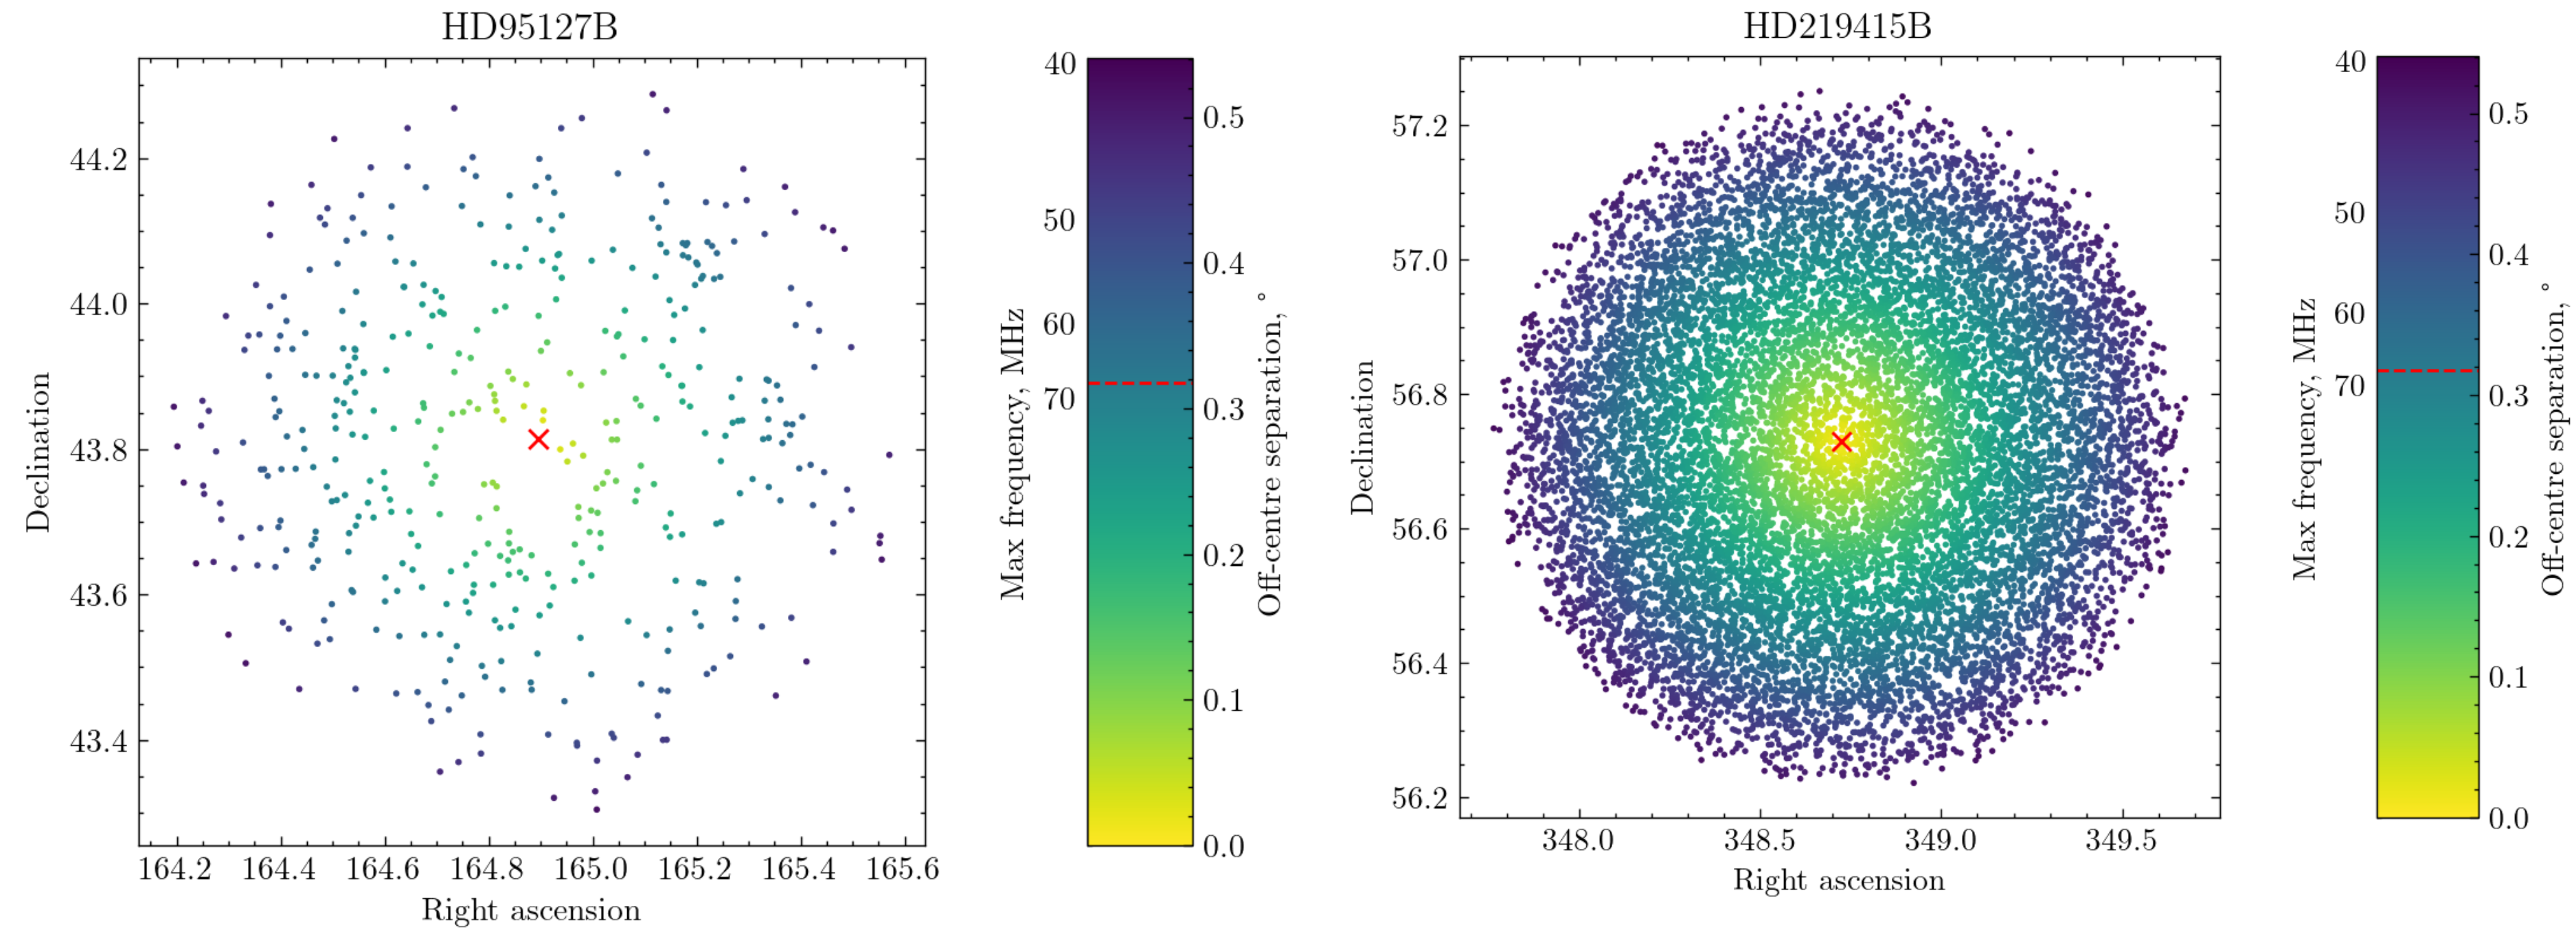
\includegraphics[width=0.95\linewidth]{chapter6/figures/NenuFAR/NenuFAR_Beam_Example.png}
    \caption{Two example pointings of the NenuFAR technosignature survey. \textit{Left}: BD+48738B, a target near the Galactic plane. \textit{Right}: GJ3942B a target off of the Galactic plane}
    \label{fig:NenuFARBeam}
\end{figure}

Here 0.32–0.54° for off-beam pointings were considered when searching the \textit{Gaia} catalogue because.... On average there were 3417 stars in each pointing at the middle of the band (47.8~MHz). The population's distribution and associated HR-diagrams can be seen in \cref{fig:NenuFARpopulation}.


\begin{figure}
    \centering
    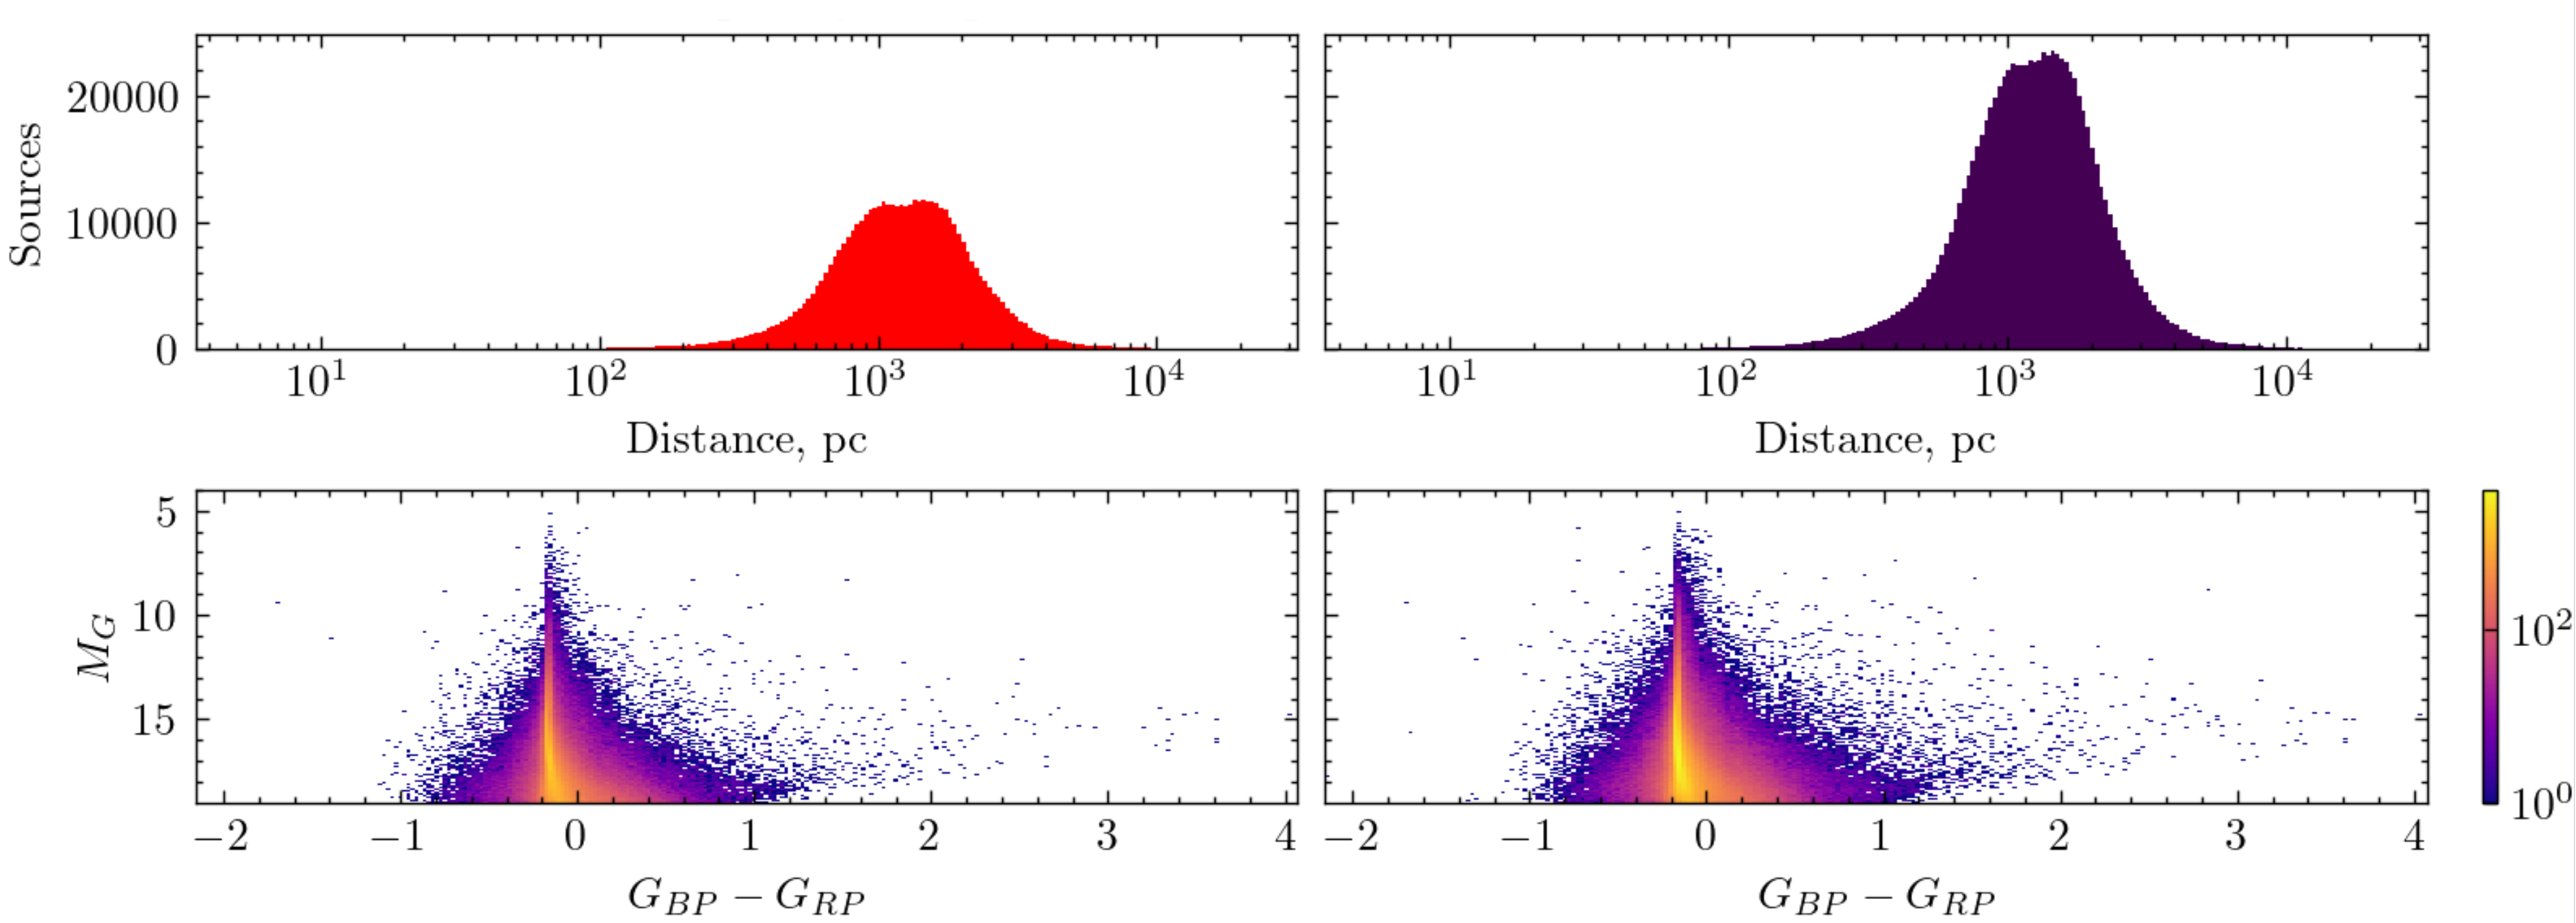
\includegraphics[width=0.95\linewidth]{chapter6/figures/NenuFAR/NenuFAR_populations.png}
    \caption{The top two panels show the distance ditribution of \textit{Gaia} sources at the bottom of the band (39.8~MHz) and the top of the band (67.7~MHz). The bottom panels show bot the bottom and top bands matching HR-diagrams. }
    \label{fig:NenuFARpopulation}
\end{figure}


Using the same method as described in \cref{sec:SETIchapter} using \cref{Eq:EIRP} and \cref{eq:modified-drake} constraints can be placed on this frequency regime. The constraint this survey placed on the fraction of narrowband emitting civilisations, $f^n_c$, using a one-sided Poisson upper limit of 95\% \citep{Gehrels:1986p10835} is shown in \cref{fig:NenuFARconstraints}.

\begin{figure}[h]
    \centering
    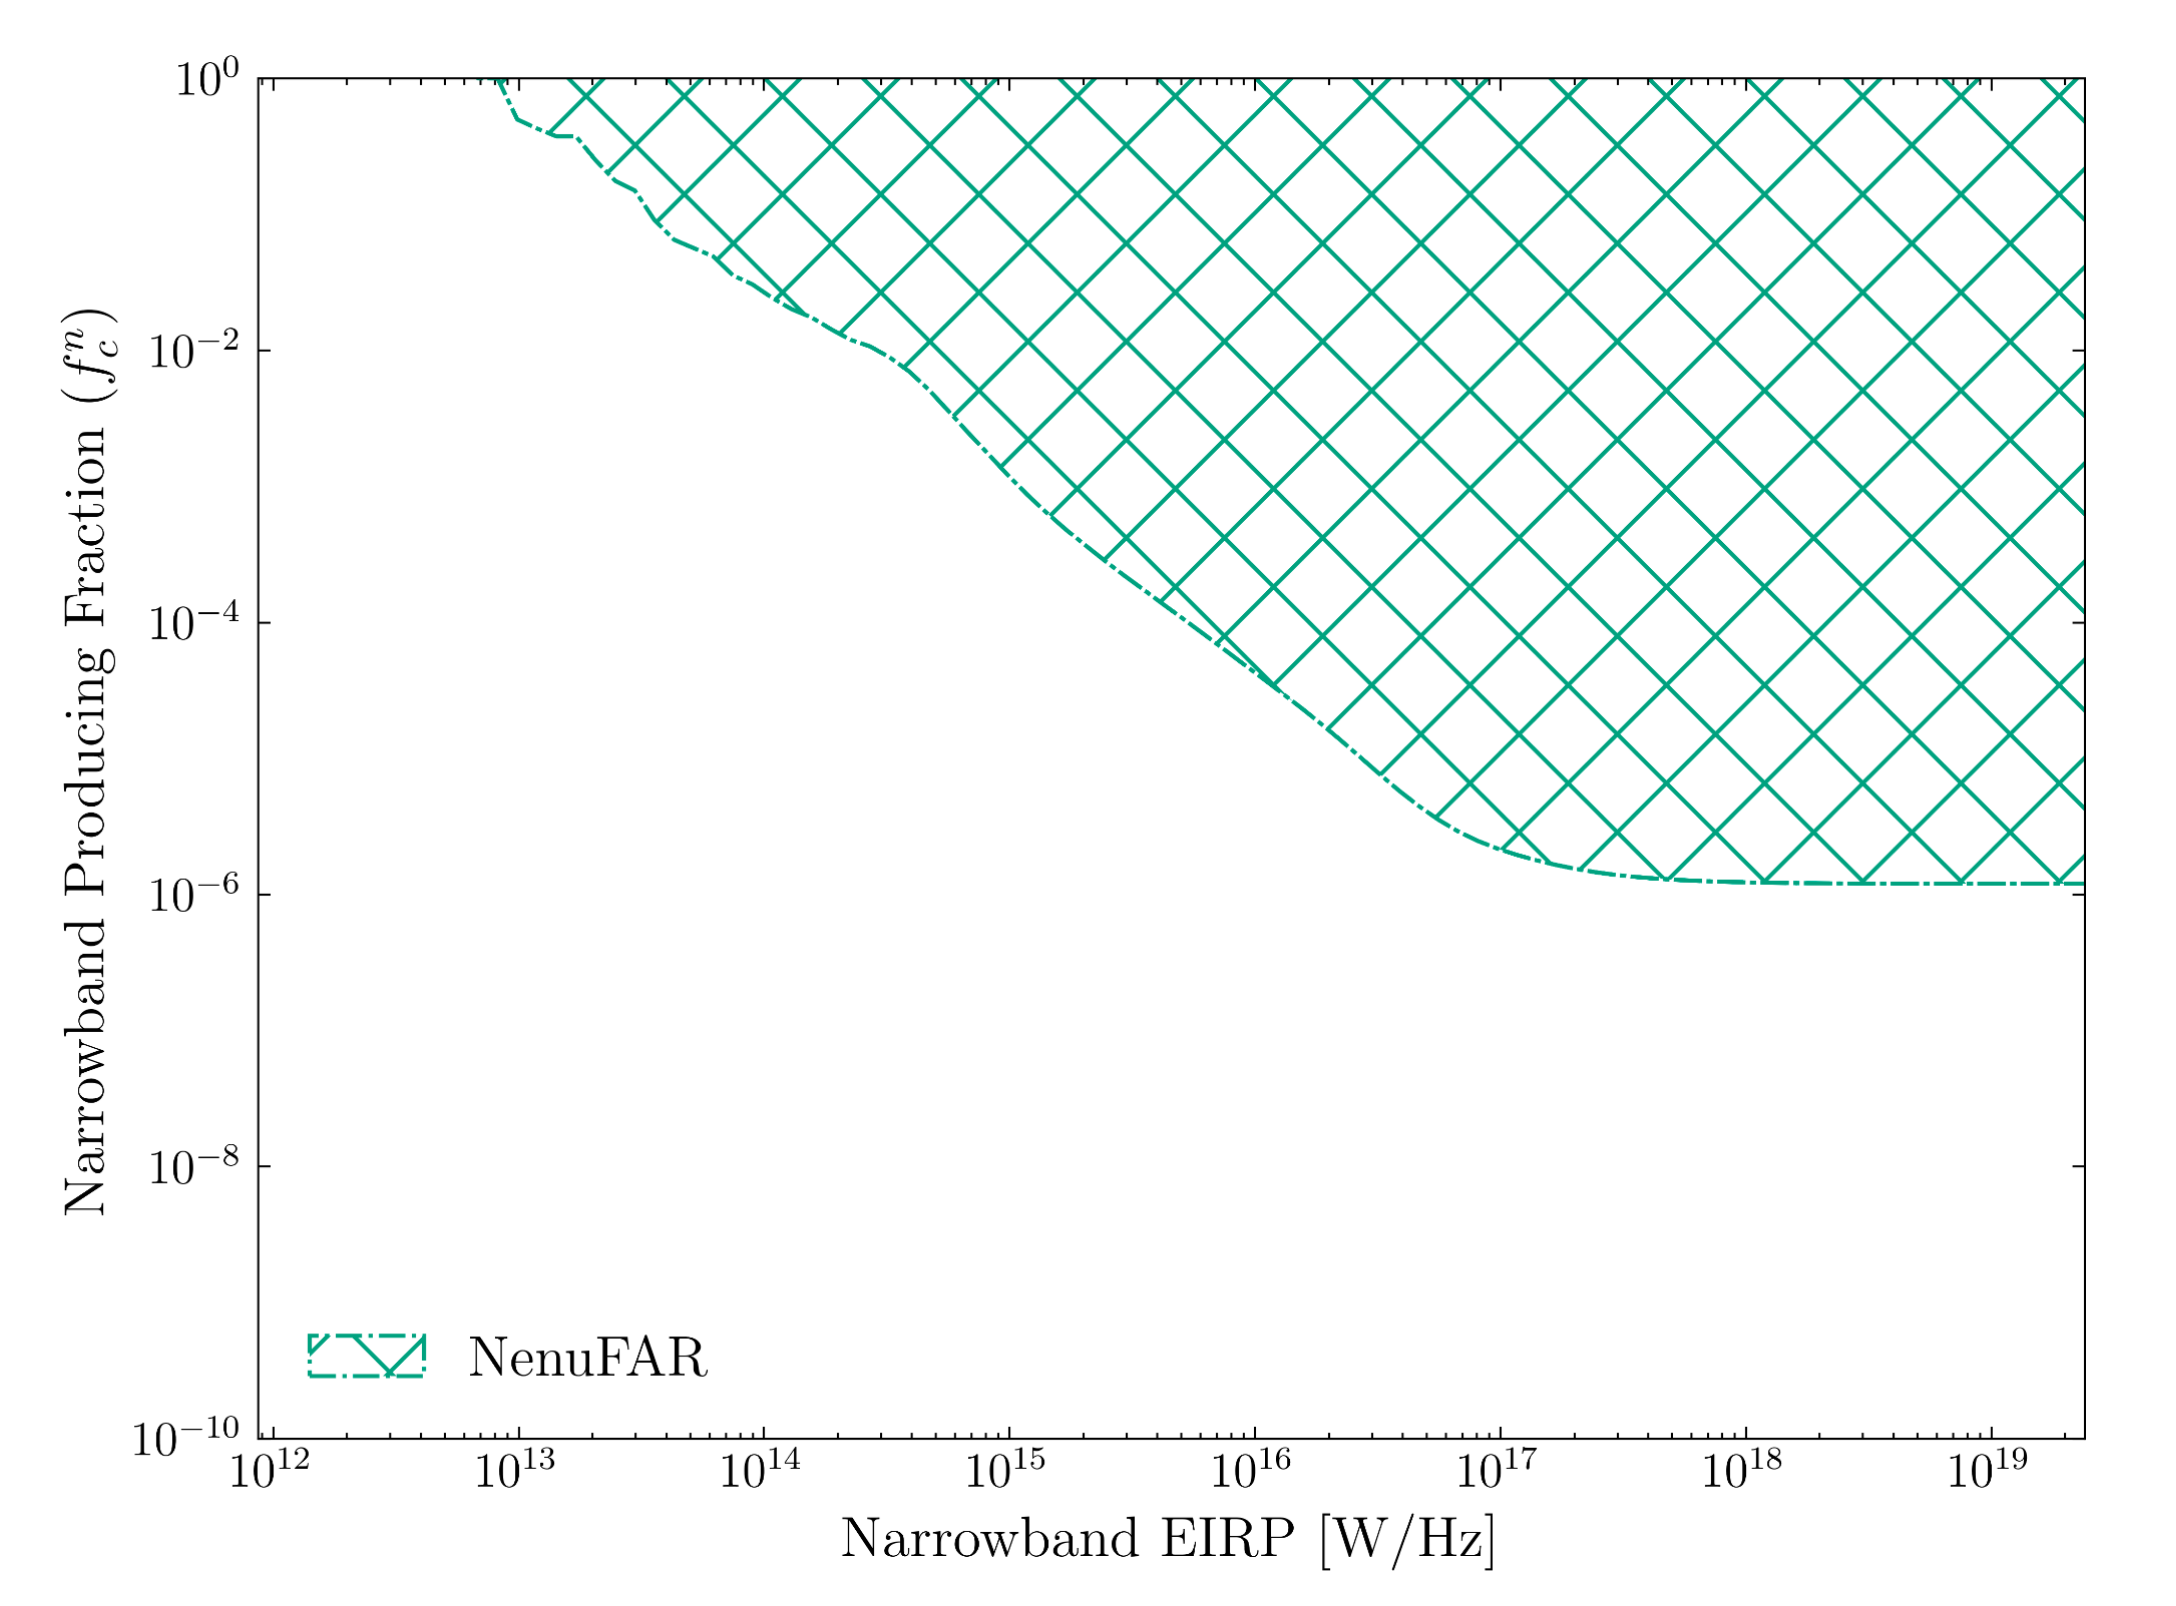
\includegraphics[width=0.75\linewidth]{chapter6/figures/NenuFAR/NenuFAR_Constraints.png}
    \caption{The fraction of stars that produce narrowband emission against the transmitter power of the total target pool. The hashed region (green) shows the constraints this survey places on a value of $f^n_c$ at 39.8–67.7 MHz.}
    \label{fig:NenuFARconstraints}
\end{figure}

Another major advancement is the development of a commensal acquisition pipeline using the SETIBK backend led by Louis Bondonneau and Cedric Dumez-Viou. This system enables automatic collection of beamformed data from virtually every NenuFAR observation conducted by collaborating scientific programs. The capability significantly increases observing efficiency by generating SETI-compatible datasets without requiring dedicated telescope time. Furthermore, real-time data reduction software based on the UnDySPuTeD backend \citep{bondonneau_pulsars_2021} has been deployed on \textsc{SETIBK} to produce science-ready products directly during observations, although additional testing and optimization are required to eliminate spectral artifacts observed at the highest frequency resolutions.

Future work focuses on completing the reduction and analysis of all collected observations and deploying an automated detection pipeline capable of identifying Doppler-drifting narrowband signals while distinguishing genuine astrophysical candidates from terrestrial interference through repeated ON/OFF observations. Additional priorities include systematic monitoring of the telescope's RFI environment using routine horizon and zenith scans, investigation of out-of-band emissions from low-Earth-orbit communication satellites such as Starlink \citep{LOFAR-Starlink}, and development of machine learning algorithms for novelty detection in SETI datasets. These improvements are expected to enhance both the sensitivity and reliability of future technosignature searches while remaining to place the most stringent constraints on the lowest frequencies for prevalence of life in the universe.

% 274 observations of confirmed GAIA exoplanets have been conducted over the span of Early Science period and the first semester of the Science period. The distribution of pointings in the Galactic plane is illustrated in Figure 1. 

% A conic search of the Gaia catalogue was conducted for each pointing of the surveyed targets within the Full Width at Half Maximum (FWHM) of the bore sight pointing. This resulted in a substantial number of targets, totalling over 3.5 million. Consistent with [2], the Gaia targets underwent filtering based on their coordinate values and distance values. These filters can be described as follows: firstly, stars with errors extending beyond the area enclosed by the FWHM were excluded.

% This resulted in a total over 868,665 targets. The change in targets across the frequency band has also been calculated. An example of two of these pointings can be seen in Figure 2. Searching the off-beam pointing for Gaia targets should theoretically double the number of targets observed in the study and will have a cascading effect on the sensitivity calculations and constraints discussed below. The subsequent step in the analysis involved comparing the sensitivity of the NenuFAR SETI survey to other surveys. This comparison was based on the following equation for Effective Isotropic Radiated Power (EIRP):